% Syslab Research Journal Template
% By Patrick White
% September 2019

% Do not edit this header
\documentclass[letterpaper,11pt]{article}
\usepackage{fullpage}
\usepackage{palatino}
\usepackage{enumitem}
\usepackage{courier}
\usepackage{graphicx}
\def\hrulefill{\leavevmode\leaders\hrule height 20pt\hfill\kern\z@}

% ------------- Edit these definitions ---------------------
\def\name{Bryan Lu}
\def\journalnum{10}
\def\daterange{11/18/19-11/25/19} % starts on Monday
\def\period{2}
% ------------------ END ---------------------------------
% Do not edit this
\begin{document}
	\thispagestyle{empty}
	\begin{flushright}
		{\Large Journal Report \journalnum} \\
		\daterange\\
		\name \\
		Computer Systems Research Lab \\
		Period \period, White
		\end{flushright}
	\hrule height 1pt

% ------ SECTION DAILY LOG -------------------------------------
\vspace{-0.8em}
\section*{Daily Log}
%Detail for each day about what you research, coded, debug, designed, created, etc. Informal style is OK.
\vspace{-0.8em}

\subsection*{Monday, November 18}
\vspace{-0.6em}
Fixed github issues and successfully pushed all work and code to TJ CSL github page. 
\vspace{-1.3em}
\subsection*{Tuesday, November 19}
\vspace{-0.6em}
Finished assigning relations to half of my test cases. I added boolean relations to \texttt{finalrelations.txt} that check whether or not points or circles were special points/circles with respect to a given triangle, and relations that check for concyclicity of points. 
\vspace{-1.3em}
\subsection*{Thursday, November 21}
\vspace{-0.6em}
Finished assigning relations to 90\% of my test cases, with some uncertainty as to how to deal with implicit relations and implicit objects present in a sentence that don't have explicit variables assigned to them. 

\vspace{-1.0em}

% ------ SECTION TIMELINE -------------------------------------
%\newpage
%\vspace{-1.7em}
\vspace{-1.0em}
\section*{Timeline}
\begin{tabular}{|p{1in}|p{2.5in}|p{2.5in}|}
	\hline
\textbf{Date} & \textbf{Goal} & \textbf{Met}\\ \hline 
	\hline 
11/4 & Create the log-linear classifier/learning algorithm and the training data, and begin testing. & I've started, but I've realized this is a rather ambitious task because I still need to finish creating my training data.\\
	\hline
11/11 & Complete a set of about 40 problems to serve as my training data set, with the correct relations. & I have the problems, but putting in the correct relations for these problems is a lot of work. \\
	\hline
11/18 & Build the model with \texttt{scikit}, tweaking previous steps as needed, and finish the necessary test cases. & I didn't have any time this week to start building the actual model, but my test cases are now more or less where I want them to be. \\
	\hline
11/25 & Build, test, and train the logistic model, given the test data and the features computed. & N/A \\
	\hline 
12/2 & Refine logistic learning model with extra methods to try to increase accuracy, and begin extracting the most likely literals. & N/A \\
	\hline 
Winter Goal & Be able to output a set of possible literals (statements) based on detected relations in the problem. & N/A \\
	\hline 
\end{tabular}


% ------ SECTION REFLECTION  ---------------------------------
\section*{Reflection}
%In narrative style, talk about your work this week. Successes, failures, changes to timeline, goals. This should also include concrete data, e.g. snippets of code, screenshots, output, analysis, graphs, etc.

I don't have very much to show this week for my work because most of it was menial work that had to get done at some point. Attached is a screenshot of what my text file of relations contains as of right now -- each problem is currently formatted so that it fits nicely on the page, with the associated relations that describe the problem below each problem. 
\begin{center}
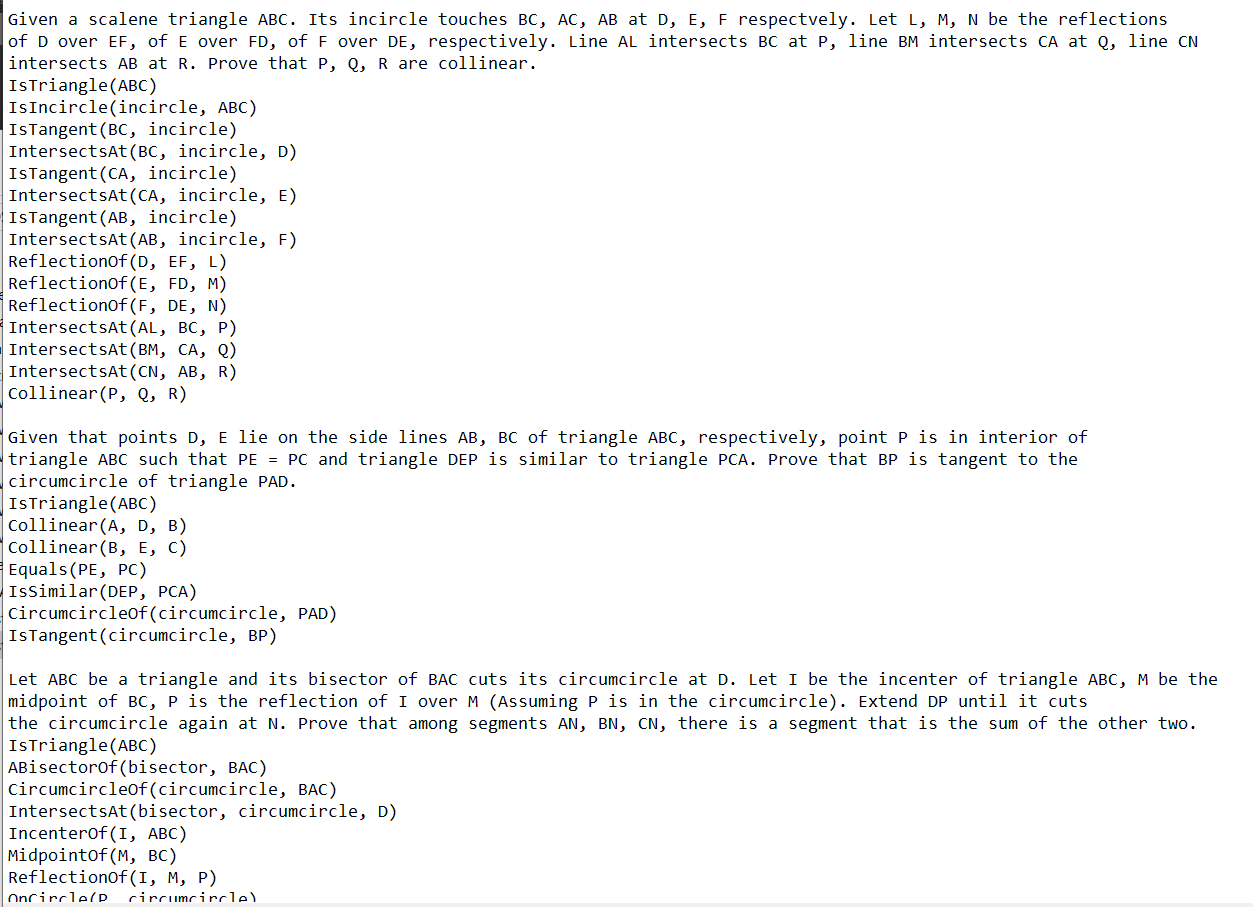
\includegraphics[scale=0.5]{testcases.png}
\end{center}
Currently, my \texttt{finalrelations} file only contains boolean relations -- that is, all of my relations currently jsut take in some number of variables and output a boolean value corresponding to whether or not that statement is true. As I have been constructing these test cases, however, I've found that having relations that output variables as well would be useful, although it would make the testing much more difficult. For example, in the second displayed problem, the circumcircle of triangle $PAD$ is relevant to the statement that is needed to be proved, although it's not given an explicit name other than ``circumcircle.'' This doesn't present too much of an issue here, but with problems that involve more than one unnamed object, there is a pretty clear opportunity for confusion to occur while checking if a relation generated by the model is correct. Hence, I think it's reasonable to add one-argument relations such as \texttt{Circumcircle(var triangle)}, which would return a variable denoting the actual circle of that triangle, in order to avoid this.

Any relations that I've been adding to my \texttt{finalrelations} file over the past week or two also need to be somehow added into my \texttt{lexicon} file, or otherwise the code won't be able to detect these important relations that need to be detected for a successful ``understanding'' of the problem. This shouldn't take long, but it is something that needs to be addressed. 
\end{document}

